\chapter{Background}
\todoStyle{go label all glossary terms!}
\label{ch2}
As computational geometry is founded on many other fields of study in both mathematics and computer science, likewise \Fors{t} also relies on the same. In this chapter, we briefly cover many theories, concepts, and frameworks across many fields of study, opting for breadth over depth, in order to focus only on the specific topics which have a direct influence on research presented in the rest of this thesis.

Section~\ref{ch2sETB} covers the elementary, theoretical basis for the mathematics utilized in the design of \fors{t}, including various topics in set theory, linear algebra, geometry, and topology. Next, Section~\ref{ch2sTDD} defines several symbols which will be used throughout the rest of this thesis while discussing in relative detail the primitives of \tdd{}, as well as the nature of discrete meshes, one-ring neighborhoods, the differences between acquired and synthetic \tdd{}, and the treatment of scalar fields as function values. Then in Section~\ref{ch2sPP}, various topics regarding the design and analysis of algorithms for parallel processing are briefly discussed.

%
%
%
%
%
%
\section{Elementary Theoretical Basis}
\label{ch2sETB}
This section discusses an abbreviated collection of the elementary, theoretical concepts that comprise the basis upon which \fors{t} was designed. These important concepts and symbols are collected into sections, including limited topics from: set theory in Section~\ref{ch2sETBssST}, linear algebra in Section~\ref{ch2sETBssLA}, geometry in Section~\ref{ch2sETBssG}, and topology in Section~\ref{ch2sETBssT}.

%
%
%
%
\subsection{Set Theory}
\label{ch2sETBssST}
A set is one of the most fundamental concepts in mathematics. Informally, a set is a collection of distinct objects, and is also itself considered to be an object. In this thesis, sets are denoted using capital, calligraphic letters, including: $\bE$, $\bF$, $\bM$, $\fM$, $\bN$, $\bP$, and $\bT$. Each of these will be defined and described in detail when introduced individually, later in this thesis. In this section, we will introduce the concepts and nomenclature used to define a set, reference special sets, determine the cardinality of a set, as well as apply membership, relational, and binary operators on sets.

%
%
\subsubsection{Set Definitions}
\label{ch2sETBssSTsssSD}
As several different sets are used throughout the remainder of the thesis, we must first discuss how it is one may define a set and its membership, including ``intensional definitions'' and ``extensional definitions''. An intensional definition uses semantic rules and symbols, where each symbol can be translated into words so that the definition may be coherently read aloud. For example,

\begin{equation}
	\bP := \left \{\:\bp_v \mid v \in \mathbb{N}, \;\text{and}\; 1\leq v \leq v_{max}\:\right \}
\end{equation}

which should be read as, ``the set $\bP$ is defined as the set of all points $\bp_v$, such that the index $v$ is a member of the set of natural numbers, and $v$ is a number from 1 to the maximum index of points in the set.''

The other option, extensional definition, is denoted by enclosing the list of members in curly brackets and optionally invoking an ellipsis (\dots) for continuing into infinity. For example,

\begin{equation}
	\mathbb{N} = \left \{\:0,\,1,\,2,\,3,\,\ldots\:\right \}
	\label{eq:definitionNaturalNumbers}
\end{equation}

which in words, means ``the set of natural numbers is the set which includes every integer from zero\footnote{In some literature, zero is excluded from the set of natural numbers.}\todoCitation{zero not in set of natural numbers} until infinity.''

It is allowed for one to list a set member two or more times in a definition. For example, $\left \{\:4,\,2,\,2\:\right \}$. However, it is identical to the set $\left \{\:4,\,2\:\right \}$ per the axiom of extensionality\todoResearch{Zermelo–Fraenkel set theory., Axiom of extensionality, logical extensionality}, which states that two definitions of sets, which differ only in that one of the definitions lists members multiple times, define the same set.

%
%
\subsubsection{Special Sets}
\label{ch2sETBssSTsssSS}
There exist some sets which are used in mathematical literature with such frequency as to demand their own standardized symbols. In this thesis\todoReference{defineSetofNaturalNumbers}, we have already encountered $\mathbb{N}$, as defined in Equation~\ref{eq:definitionNaturalNumbers}, which denotes the set of all natural numbers, but more often we will use the set of all real numbers $\mathbb{R}$, which can be described as ``the set of all positive or negative, rational or irrational numbers, including zero''. In short, any number which is not imaginary. This special set, is also usually written with a superscript denoting a specific dimensionality, as in $\bR{3}$ for three-dimensional data.

%
%
\subsubsection{Cardinality}
\label{ch2sETBssSTsssC}
Many times throughout this thesis, we reference the cardinality of set, which simply means the total count of its membership, and is denoted by two enclosing bars. For example, if $\bM$ is defined as the set $\left \{\,\bP,\,\bT\right \}$, then $|\bM\,| $, read the cardinality of $\bM$, equals two. Cardinality is a very important metric\footnote{Closely related to cardinality is the concept of a census which, as used in this thesis, is devoid of any special symbol, but is defined as the total count of all members, of every member, of a multidimensional set or family of sets. An algorithm for computing a census is presented in Section~\ref{ch5sBNPssPVBN}.} for the research presented in this thesis. For example, in reasoning about the number of faces in a mesh or discussing the count of points in a neighborhood.

%
%
\subsubsection{Membership \& Relational Operators}
\label{ch2sETBssSTsssMRO}
If an object is said to be a member of a set, it is written with the symbol $\in$ and expressed as either ``belonging to'', or ``being an element of'', or simply being ``in'' the set. Similarly, a set may be the subset of another set, written with the symbol $\subseteq$, meaning that every member of the first set is also a member of second set. A superset works exactly in reverse, written with the symbol $\supseteq$, it is the identity where every member of the second set is also a member of first set.

In mathematical notation, the membership and relational operators are written as\footnote{The negative operators also exists as $\notin$, $\nsubseteq$, and  $\nsupseteq$}

\begin{align}
	B & \in \left \{A,\,B,\,C\right \} \\
	\left \{A,\,B\right \} & \subseteq \left \{A,\,B,\,C\right \} \\
	\left \{A,\,B,\,C\right \} & \supseteq \left \{A,\,B\right \}
\end{align}

Furthermore, a ``family of sets'' is defined as a multidimensional set, or rather, a set of sets. In general, each member of a family of sets is a set which shares some common quality with the other members of the family. For example, in Section~\ref{ch2sTDDssORN} we will define the set of sets of neighbors as a family of sets, with each member being a set of points comprising a single neighborhood. In this example, it would also be correct to reference to it as simply, a set of neighborhoods.

%
%
\subsubsection{Binary Operations}
\label{ch2sETBssSTsssBO}
Among all the basic binary operations one can perform on a set\footnote{which are the union, intersection, complement, and Cartesian product.}, in this thesis, we exclusively use the union operation, denoted as $\cup$, whose output is the set of all objects that are members of either set, or both. For example:
\todoStyle{all footnotes need punctuations}

\begin{equation}
	\left \{0,\,1,\,2\right \} \cup \left \{2,\,3,\,4\right \} = \left \{0,\,1,\,2,\,3,\,4\right \}
\end{equation}

Also noteworthy, are the commutative and associative properties of the union\todoCitation{associatePropertyOfUnions} operation, which are analogous to the similarly named properties of the addition operator for scalar values. These properties say that the order of the sets, and how the sets are grouped, do not change the final result of the operation\todoCitation{properties of operations, link in notes}, for example:
%Halmos, P. R. (2013-11-27). Naive Set Theory. Springer Science & Business Media. ISBN 9781475716450.

\begin{equation}
\begin{aligned}
	\big( \left \{0,\,1\right \} \cup \left \{1,\,2\right \} \big) \cup \left \{3,\,4\right \} & = \left \{0,\,1\right \} \cup \big( \left \{3,\,4\right \} \cup \left \{1,\,2\right \}\big) \\
	& = \left \{0,\,1\right \} \cup \left \{1,\,2\right \} \cup \left \{3,\,4\right \} \\
	& = \left \{0,\,1,\,2,\,3,\,4\right \}
	\label{eq:ascAndComPropertiesOfUnions}
\end{aligned}
\end{equation}

The commutative and associative properties of the union operation are exploited in both Algorithm~\ref{alg:serialBuildNeighborhoods} and Algorithm~\ref{alg:parallelBuildNeighborhoods} in order to reduce the complexity of the computations required to ultimately convolve \Fors{t}. In the next section, we will introduce another field of study in mathematics which is essential to the research of this thesis: linear algebra.

%
%
%
%
\subsection{Linear Algebra}
\label{ch2sETBssLA}
Nearly as fundamental as set theory, linear algebra is the branch of mathematics which studies the different methods and representations which may concern a line, including: sets of equations, matrices, transformations, vector spaces, norming functions, et cetera. Linear algebra is used in almost all scientific domains that require the use of mathematics, including geometry and scientific computing, and also provides the symbols and concepts for performing blocks of operations in parallel~\cite{Weisstein19i}. In this section, we will briefly introduce only the major concepts used in our research: position vectors, the subtraction of two vectors, and computing the L2-norm of a vector.
\todoStyle{put all citations BEFORE punctuation}

%
%
\subsubsection{Position Vectors}
\label{ch2sETBssLAsssPV}
\todoCitation{position vector}
The concept of position vectors is of paramount importance to nearly all of the calculations which must be performed by the \fors{t}, because the research in this thesis is focused on the efficient convolution of the filter over a discrete manifold embedded in 3D-space, with each point being represented by a set of three Cartesian coordinates, equating points with position vectors.

As in \tdd{}, all position vectors are represented by a set of Cartesian coordinates with cardinality matching that of the dimensionality of the Euclidean space in which it is embedded. For example, in Section~\ref{ch2sTDDssP} we say that a point can also be called a position vector, so if we are given a point in $\bR{3}$, it is defined by the three Cartesian coordinates $x$, $y$, and $z$. ``Cartesian'' refers to the French scholar, René Descartes~\cite{EB1}, and ``Euclidean'' refers to Euclid of Alexandria, the Ancient Greek mathematician~\cite{EB2}.

Figure~\ref{fig:definePositionVector} provides three examples of why a point may be called a position vector. Any set of coordinates has an implied direction pointing away from the origin, which in $\bR{3}$ is located at $(0, 0, 0)$. In (a), the point $\bp_a$ is in $\bR{1}$ and located at at coordinate $(4)$, which is at a distance of $4$ units away from the origin. In (b), the point $\bp_b$ is in $\bR{2}$ and located at at coordinates $(4,\,4)$, which is at a distance of $4\sqrt{2}$ units away from the origin. In (c), the point $\bp_c$ is in $\bR{3}$ and located at coordinates $(4,\,4,\,4)$, which is at a distance of $4\sqrt{3}$ units away from the origin\footnote{The lengths in this example increase with each additional dimension: $4 < 4\sqrt{2} \approx 5.657 < 4\sqrt{3} \approx 6.928$}. This concept extends to any Euclidean space $\bR{n}$.

\begin{figure}[ht]
\ffigbox
	{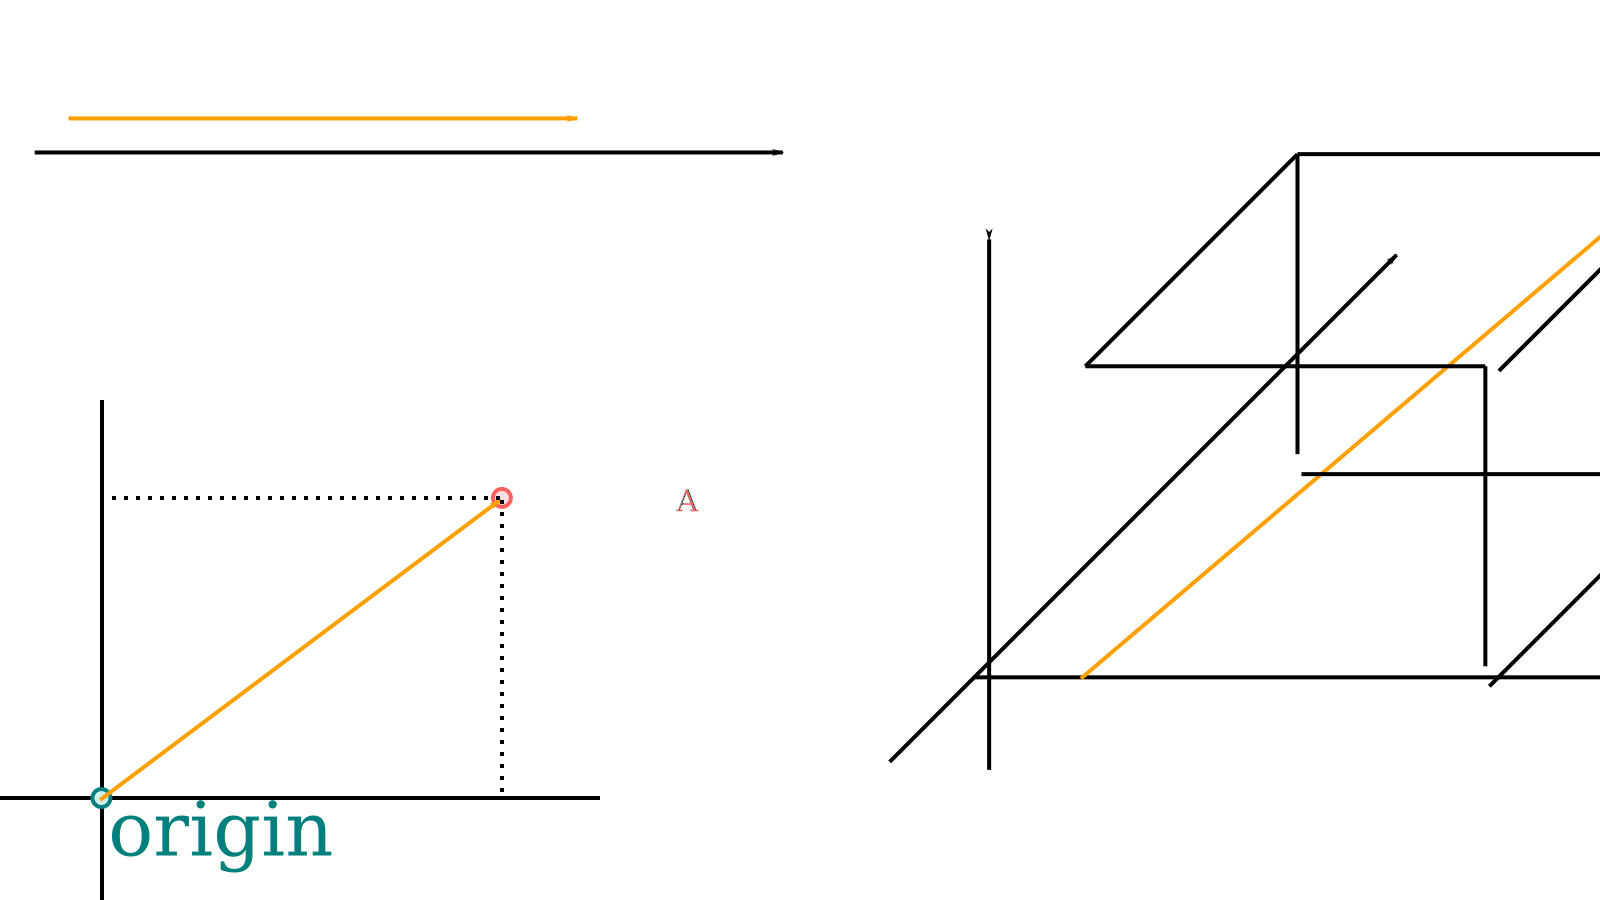
\includegraphics[width=1.0\linewidth]{figures/definePositionVector.png}}
	{\caption[Thre Examples of Position Vectors]{Three examples of position vectors shown as arrows in sand color pointed from the origin in teal color to the points in coral color: (a) $\bp_a$ in $\bR{1}$ at coordinate $(4)$ with length 4, (b) $\bp_b$ in $\bR{2}$ at coordinates $(4,\,4)$ with length $4\sqrt{2}$, (c) $\bp_c$ in $\bR{3}$ at coordinates $(4,\,4,\,4)$ with length $4\sqrt{3}$. The origins are located at $(0)$, $(0,\,0)$, and $(0,\,0,\,0)$ respectively.}\label{fig:definePositionVector}}
\end{figure}

%
%
\subsubsection{Subtracting Two Vectors}
\label{ch2sETBssLAsssS2V}
Among the various binary operators with which one could operate on vectors, this thesis is primarily concerned with subtraction, because it will be used to not only calculate the distance between each pair of adjacent points in the mesh, but also to interpolate and extrapolate the function values during the calculations of the \wmfv{s} described in detail in Sections~\ref{ch3sIE}~and~\ref{ch3sWM}.

In order to use the subtraction operator on two vectors in the same Euclidean space, one must simply subtract each component element-wise.~\cite{Weisstein19j} For example, given two points in $\bR{3}$, $A$ and $B$, the difference is calculated as

\begin{equation}
	A - B = (A_x - B_x,\,A_y - B_y,\,A_z - B_z)
	\label{eq:vectorSubtraction}
\end{equation}

This results in the single set of new coordinates, $\{C_x, C_y, C_z\}$, which both represents the point $C$ located there, or the position vector pointed from the origin to there.

%
%
\subsubsection{L2-norm}
\label{ch2sETBssLAsssL2N}
The L2-norm may be seen elsewhere in the literature abbreviated as $L^2$ or $\ell^2$, or perhaps called the ``Euclidean norm'' or ``Euclidean distance''. It is so named because it is the ordinary, straight line distance between two points in Euclidean space, and in the case of a position vector $\bP$ in $\bR{3}$, those two points are the origin at $(0, 0, 0)$ and $\bp$ at the coordinates $\{\bP_x,\,\bP_y,\,\bP_y\}$~\cite{Weisstein19h}.

The purpose for calculating the L2-norm of a vector is to determine the ordinary, uni-dimensional length of the vector, regardless of the dimensionality of Euclidean space in which it is embedded. The significance of this distinction can be seen in Figure~\ref{fig:definePositionVector}; despite having all coordinates exclusively set to $4$, the position vector on (a) is of length $4$, in (b) it is of length $4\sqrt{2} \approx 5.657$, and in (c) it is of length $4\sqrt{3} \approx 6.928$.

To determine the length of a vector, one can use the following equation for calculating the L2-norm,

\begin{equation}
	|\bp| \enspace=\enspace \|\bp\|_2 \enspace=\enspace \sqrt{x^2 + y^2 + z^2 + \ldots + n^2} \enspace:\enspace \bp \in \bR{n}
	\label{eq:l2norm}
\end{equation}

In this thesis, the L2-norm is denoted using the abbreviated symbol $|\cdot|$. Please be aware of the similar notation for the cardinality of a set $|\bP|$. While the matching symbols do represent somewhat similar concepts, cardinality is the count of elements in the set, but the L2-norm of a vector is calculated as in Equation~\ref{eq:l2norm}.~\cite[p.~26]{Mara12}

%
%
%
%
\subsection{Geometry}
\label{ch2sETBssG}
As vast and encompassing as the field of geometry is, in this section, we will only introduce the few concepts which are of paramount importance for \fors{t}, including: geodesic discs for ensuring a consistent filter widow size for the duration of each convolution in Section~\ref{ch3sSEL}, the characteristics of a circle sector to be used in calculating the area and center of gravity in Section~\ref{ch3sACG}, as well as interpolation and extrapolation for calculating the \wmfv{s} in Section~\ref{ch3sWM}.
\todoResearch{weighted averaging using density}
\todoResearch{static filter window size importance}

%
%
\subsubsection{Geodesic Discs}
\todoStyle{Why periods after figure numbers, but not section numbers?}
\label{ch2sETBssGsssGD}
Geodesy, the term from which geodesic discs get their name, is defined differently in many fields.\todoCitation{geodesy} A geodesic, as defined in the original sense, was the shortest route between two points on the Earth's surface; so a straight line distance in curved space. In this thesis, we use the term geodesic disc to mean the surface area on a manifold, encompassed by a circle with a given radius, which itself is also embedded in $\bR{3}$, and reference to this disc with the symbol $\bO$.

The significance is that one may treat similarly all adjacent faces in a neighborhood of a non-planar mesh as if they were planar, greatly simplifying the required mathematics involved. It also becomes possible to ensure a consistent filter window size for the duration of each convolution of \fors{t}, despite that given the nature of acquired \tdd{} as discussed in Section~\ref{ch2sTDDssAVS3}, each adjacent face likely exists on a different plane in $\bR{3}$ than its neighbor. Also, from the geodesic disc we derive the circle sectors which are described in detail in the next section.
\todoResearch{static filter window size importance}
\nomenclature[aa]{$\bO$}{a geodesic disc}%
\nomenclature[ab]{$\bO_v$}{a specific geodesic disc centered about the point $\bp_v$}%

%
%
\subsubsection{Circle Sectors}
\label{ch2sETBssGsssCS}
A circular sector, or circle sector, is the portion of a disc enclosed by two radii and an arc. In general, the larger area is known as the major sector, however \fors{t} is only concerned with the area of the other, smaller area, known as the minor sector. This is a natural way to partition a geodesic disc embedded in $\bR{3}$, where each sector can be delineated by the border of two triangular faces which likely exists on different planes.\todoReference{figure of geodesic disc in 3d, once made} Going forward, the minor circle sector will be abbreviated as just ``the circle sector'', or even more simply, ``the \gls{sector}''
\todoReword{replace all occurrences of circle sector with glossary term sector, consider adding the to glossary term}, and will be denoted as $\bs$, or $\bs_i$ in reference to a specific circle sector, as described in Section~\ref{ch3sSEL}.%
\nomenclature[ba]{$\bs$}{a circle sector}%
\nomenclature[bb]{$\bs_i$}{a specific circle sector of geodesic disc $\bO_v$}%

As the sector can be described entirely by the central angle $\alpha$ and the circle's radius\footnote{$\ell_{a,b}$ was chosen to represent the radius instead of the much more common $r$, because in \tdd{}, edges are not stored, yet distances between points can be calculated as shown in Section~\ref{ch2sTDDssEL}.} $\ell_{a,b}$, the area of the sector can be given as

\begin{equation}
	A = \pi \ell_{a,b}^2\frac{\alpha}{2\pi} = \frac{\ell_{a,b}^2\alpha}{2}
	\label{eq:areaOfCircleSector}
\end{equation}

because of the fact that in radians, the ratio of a sector's central angle $\alpha$ to the complete angle of the circle $2\pi$, is equal to the ratio of that sector's area to the area of the whole circle~\cite{Weisstein19d}.%
\nomenclature[bc]{$A$}{an area of a circular sector}%

%
%
\subsubsection{Center of Gravity}
\label{ch2sEBTssGsssCG}
Along with area, the other important characteristic of a circle sector for \fors{t} is the centroid, or center of gravity, which is used in both Algorithms~\ref{alg:serialConvolveFilter}~and~\ref{alg:parallelConvolveFilter} in order to calculate the \wmfv{s}, by serving as the location to which the function values are interpolated, the operation which is discussed in the next section.

The center of gravity is so named, because it is the point where the sector would balance on a pin\footnote{given that it had been bestowed a volume with uniform density.}. The center of gravity $\bc$ is calculated as the distance from the center point $\bp_a$, along the line which bisects the central angle $\alpha$, and is given by

\begin{equation}
	\check{\ell} := \frac{4\:\gelm\:\sin(\frac{\alpha_i}{2})}{3\,\alpha_i}
	\label{eq:ch2distToCoG}
\end{equation}%%
\nomenclature[ca]{$\bc$}{the center of gravity of circle sector $\bs_i$}%
\nomenclature[cb]{$\check{\ell}$}{the distance from $\bp_0$ to $\bc$}%

In the Figure~\ref{fig:circleSector}, a circle sector is produced by the points $\bp_a$, $\bp_b$, and $\bp_c$, has the central angle $\alpha$ which is bisected by a dotted line, and $\ell_{a,b}$ representing the length between points $\bp_a$ and $\bp_b$, which is equal radius of the circle. Also shown, is the center of gravity $\bc$, as well as $\check{\ell}$, the distance to $\bc$ from the center point $\bp_a$.

\begin{figure}[ht]
\ffigbox
	{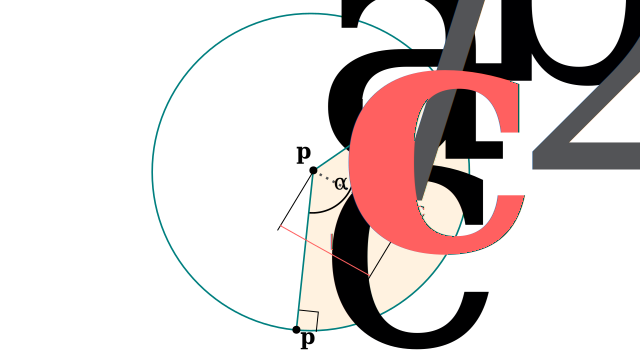
\includegraphics[width=0.6\linewidth]{figures/circleSector.png}}
	{\caption[A Circle Sector in Detail]{The circle sector produced by points $\bp_a$, $\bp_b$, and $\bp_c$, with $\alpha$ as the central angle bisected by a dotted line, and $\ell_{a,b}$ as the length between points $\bp_a$ and $\bp_b$, which is equal to the radius of the circle. Also labeled is the center of gravity $\bc$ as well as the distance from the center point $\bp_a$ to $\bc$, drawn in a coral color as $\check{\ell}$}\label{fig:circleSector}}
\end{figure}

The line which bisects the central angle of a circle sector, while not used explicitly in calculations, is an important concept for much of the computations used by \fors{t}, as will be seen in Chapter~\ref{ch4}. Therefore, we make a special note here that the abbreviated, ``\gls{bisectingLine}'', indeed refers to this line which splits the circle sector and its central angle $\alpha$ into two equivalent halves.

%
%
\subsubsection{Interpolation \& Extrapolation}
\label{ch2sETBssGsssIE}
Simply stated, interpolation is a method of constructing new data points within the range of a discrete set of known data points, such as those points found in the discrete manifolds of \tdd{}. There exist a large variety of methods for interpolating different kinds of data\todoCitation{different kinds of interpolation}, but in this thesis, we will only consider linear interpolation, which is simple to calculate\footnote{however can become imprecise in relation to the square of the distance between the data points.}\todoCitation{footnote:error of linear interpolation} and can be extended for n-dimensions\todoCitation{n-dimensional linear interpolation}.

Given the two data points in $\bR{2}$, $(x_a, y_a)$ and $(x_b, y_b)$, we can calculate the $y_c$ coordinate of a third point located along a straight line drawn between the first two points, while also having the coordinate $x_c$, as

\begin{equation}
	y_c = y_a + (y_b - y_a) \frac{x_c - x_a}{x_b - x_a}
	\label{eq:interpolationGeneral}
\end{equation}

To elaborate the concept of interpolation, now consider the two points $(1, 2)$ and $(5, 1)$, then find the $y$ coordinate of a point between them, located at the intersection of the line which contains the first two points and $x = 3$.

\begin{align}
	y_c & = 2 + (1 - 2) \frac{3 - 1}{5 - 1} \\
	& = 2 + -1 \frac{2}{4} \enspace = \enspace  1.5
	\label{eq:interpolationSpecific}
\end{align}

Therefore, we interpolate the value halfway between the two given points to be $(3,\,1.5)$, which is halfway between as expected, and illustrated in Figure~\ref{fig:interpolation}.

Conversely, extrapolation is a method for constructing new data points \textit{outside} the range of a discrete set of known data points. The process of linear extrapolation is equivalent\footnote{The difference between interpolation and extrapolation is largely an academic one, owing primarily to the lack of boundaries and increasing error rates associated with extrapolation.} to linear interpolation; namely, first calculating the line between two points, then calculating the $y$ coordinate of a third point at a new value of $x$, the latter of which will be either greater than or less than both of the first two points.

As illustrated by Figure~\ref{fig:interpolation}, the similarities and differences between the processes of interpolation and extrapolation become even more intuitive when seen graphically, where having chosen the two points $\bp_a$ and $\bp_b$, a third point $\bp_c$ is interpolated between the two points, while the fourth point $\bp_d$ is extrapolated outside their domain.

\begin{figure}[ht]
\ffigbox
	{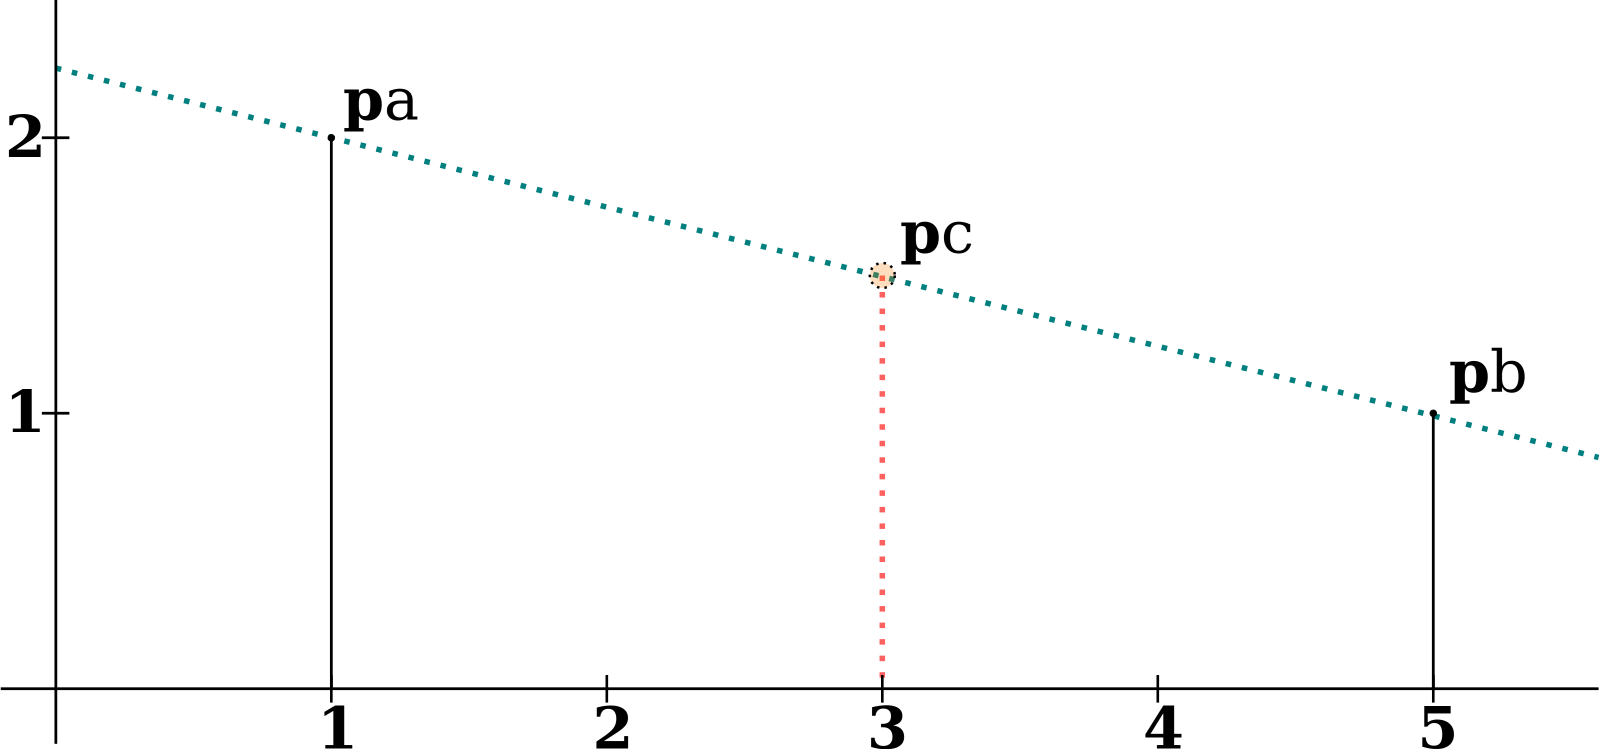
\includegraphics[width=1.0\linewidth]{figures/interpolation.png}}
	{\caption[Interpolation and Extrapolation in $\bR{2}$]{The point $\bp_c$ is interpolated as the value between $\bp_a$ and $\bp_b$, while the fourth point $\bp_d$ is extrapolated outside their domain}\label{fig:interpolation}}
\end{figure}

Later in this thesis, we will use both interpolation and extrapolation together in order to calculate the \wmfv{s} at the center of gravity of circle sectors, so that the function values may be weighted fairly in regards to their distance to the other points in the one-ring neighborhood, as discussed in detail in Section~\ref{ch3sIE}.

%
%
%
%
\subsection{Topology}
\label{ch2sETBssT}
Topology is the mathematical study of the properties of space that are preserved through deformations, twistings, and stretchings of objects\footnote{but not tearing or gluing.}. Topology developed as a field of study from geometry and set theory through analysis of concepts such as space, dimension, and transformation. For example, a circle is topologically equivalent to an ellipse, because it can be deformed by stretching.~\cite{Weisstein19c}

Of all the major concepts studied in topology, this thesis is only concerned firstly with manifolds, as \tdd{} is composed primarily of two-dimensional discrete manifolds embedded in three-dimensional space, and secondly, neighborhoods, which are the general concept from which one-ring neighborhoods are derived, thus being the basis upon which \fors{t} is founded.

%
%
\subsubsection{Manifolds}
\label{ch2sETBssTsssM}
A manifold is a topological space that is locally, but possibly not globally, Euclidean; a concept that is central to many parts of geometry because it allows complicated structures, such as the triangle mesh, to be described and understood in terms of the simpler, local topological properties. Expressed another way, this means that a manifold is an $n$D-subset of an Euclidean space $\mathbb{R}^{>n}$~\cite[p.~199]{Mara12}. For example, 1-dimensional manifolds in $\mathbb{R}^{2}$ include lines and circles, and 2-dimensional manifolds in $\mathbb{R}^{3}$, also called surfaces, can include commonly-known shapes such as the plane, the sphere, and the torus, but also of prime importance for this thesis, the triangle mesh.

The significance to our research is that each convolution of \fors{t} is comprised of calculations of the \wmfv{s} at the central point of a one-ring neighborhood, having weighted the function values in relation to the distance between each neighbor, and because those distances are uniformly dissimilar in acquired \tdd{}\todoCitation{tdd{} is not regular}, maintaining a consistent filter window size is only accomplished by defining the geodesic disc, which exists on the manifold defined by the mesh. Therefore, as mentioned in Section~\ref{ch2sETBssGsssGD} and discussed in more detail in Chapter~\ref{ch4}, the weights may be calculated sector-wise, as if all sectors were on the same plane, greatly reducing the complexity of the entire procedure.

%
%
\subsubsection{Neighborhoods}
\label{ch2sETBssTsssN}
A neighborhood is also one of the basic concepts of topology. Intuitively speaking, a neighborhood of a point is a set of points containing that point, where one can move in any direction without leaving the set. While determining the neighborhood is trivial for uni-dimensional manifolds\footnote{where each neighborhood only consists of a point, and the two points to either side of it on the line.}, and relatively simple for regular two-dimensional manifolds\footnote{such as with a 2D-image, whose pixels have at most four neighbors in orthogonal directions with a geometric distance of 1, as well as four neighbors at the diagonal directions with a geometric distance of $\sqrt{2}$.}, determining the neighborhood becomes more complicated for irregular surfaces like those found in \tdd{}. With those surfaces, one must determine the set of neighbors using the associations that define the triangular faces; the details of which are covered in detail in Section~\ref{ch2sTDDssORN}, once the other necessary topics regarding \tdd{} have already been discussed.

Figure~\ref{fig:neighborhoods} illustrates the differences among one-ring neighborhoods in different kinds of manifolds: (a) is a regular square mesh as with pixels of a digital image, (b) is a regular triangle mesh, as in a hexagonal tessellation, and (c) shows two very different neighborhoods in a single, irregular triangle mesh typical of acquired \tdd{}. In particular, notice in (c) the completely arbitrary shape and size of the one-ring neighborhoods found in the irregular triangle mesh; even the number of neighbors varies widely. From this observation, came much of the motivation behind \fors{t}.

\begin{figure}[ht]
\ffigbox
	{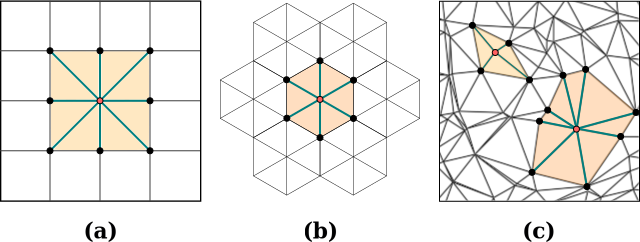
\includegraphics[width=1.0\linewidth]{figures/neighborhoods.png}}
	{\caption[One-Ring Neighborhoods in Regular and Irregular Meshes]{One-ring neighborhoods in (a) a regular square mesh, as in pixels of a digital image (b) a regular triangle mesh, as in a hexagonal tessellation (c) an irregular triangle mesh, typical of acquired \tdd{}.}\label{fig:neighborhoods}}
\end{figure}

%
%
%
%
%
%
\section{\tdd}
\label{ch2sTDD}
The data upon which one convolves \fors{t} is called \tdd\todoCitation{\tdd{} name origin, BB82 from Mara12}. As described in Section~\ref{ch2sTDDssDM}, \tdd{} consists primarily of a single mesh $\bM$, which is composed of $\bP$, a set of points, and the set $\bT$, consisting of triangular faces, each to be covered in Sections~\ref{ch2sTDDssP} and~\ref{ch2sTDDssF} respectively. As discussed in Section~\ref{ch2sTDDssAVS3}, \tdd{} also comes in two distinct flavors depending on its origin: acquired or synthetic. The data can also include a texture map and other various types of information stored as scalar or vector fields, which is elaborated on in~\ref{ch2sTDDssFV}.

%
%
%
%
\subsection{Points}
\label{ch2sTDDssP}
A point $\bp$ is the most primitive element of \tdd{}. ``Point'' is the abbreviated form of ``measuring point'', and is also known in other fields of study as a vertex, or a position vector $\bR{3}$\todoCitation{other names for a point}. A point is defined by the 3-dimensional Cartesian coordinates $x$, $y$, and $z$, and in \tdd{}, points are generally unique and not required to be in any particular order. In this thesis, a point is addressed using several different subscripts, depending on the context.

In this thesis, when referring to a point in $\bP$, $v$ is used as the globally unique index; the index with which we can define the set

\begin{equation}
	\bP := \left \{\:\bp_v \mid v \in \mathbb{N}, \;\text{and}\; 1\leq v \leq v_{max}\:\right \}
	\label{eq:defineSetOfPoints}
\end{equation}

where $v_{max}$ is the maximum index\footnote{\label{indicesFootnote}Beginning indices with 1 is significant because of the discordant conventions between addressing the first element of a data structure with 0 in programming languages, such as C++ and python, versus addressing first elements with 1, as is the standard for mathematical literature. Because this thesis should indeed be considered mathematical literature, we will always start indices at 1, and only use index 0 for special cases. For example, $\bp_0$ is used in Chapter~\ref{ch4} to represent the center point of the one-ring neighborhood.} of points in the data, and is equivalent to the cardinality of the set of points $|\bP|$.%
\nomenclature[ea]{$\bP$}{the set of points $\bp_v$ in $\bM$}%
\nomenclature[eb]{$\bp_v$}{a specific point in $\bP$}%

Otherwise, when referencing to a point within a particular face or neighborhood, the three corners can be referenced indirectly\footnote{or even more generally, as $\bp_a$, $\bp_b$, and $\bp_c$ in the case of Equation~\ref{eq:defineEdgeLengthFace}, or in the case of a nested loop: as $\bp_j$ and $\bp_{\sjpo}$ in Algorithms~\ref{alg:serialConvolveFilter}~and~\ref{alg:parallelConvolveFilter}.} as $\bp_i$, $\bp_{\sipo}$, and $\bp_{\sipt}$, or directly as $\bp_0$\footref{indicesFootnote}, $\bp_1$, $\bp_2$, etcetera.~\cite[p.~25]{Mara12}%
\nomenclature[ec]{$\bp_i$}{also $\bp_{\sipo}$, and $\bp_{\sipt}$; one of three indirectly referenced points comprising a face}%

%
%
%
%
\subsection{Faces}
\label{ch2sTDDssF}
Faces are another primitive element of \tdd{}. As we are working exclusively with triangular meshes~\cite[p.~26]{Mara12}, we define a face $\bt$ by the set of three distinct points, which we will index in clockwise order\footnote{It is worth mentioning here that many software packages, such as the GigaMesh Framework~\cite[p.~89]{Mara12}, may expect counter-clockwise ordering of indexes. This is significant because the ordering provides an orientation by which visualization software can apply texture and/or lighting. The only mathematical significance of the ordering is the sign of the area of a face, and totally inconsequential when the absolute value is expected, as shown by~\cite[p.~2]{Braden86}. This is yet another example of the difference between the conventions of mathematical literature versus those of computer science. And again, because this thesis should indeed be considered mathematical literature, we will continue to follow the conventions of mathematical literature.}~\cite[p.~4]{Mara17}.
\todoResearch{does the "right-hand-rule apply here?"}

\begin{equation}
	\bt := \left \{\,\bp_a,\,\bp_b,\,\bp_c\right \} = \left \{\,\bp_1,\,\bp_2,\,\bp_3\right \}
	\label{eq:defineFaces}
\end{equation}

With the introduction of faces comes the concept of adjacency. A face $\bt_i$ is said to be \gls{adjacent} to another face $\bt_j$ if, and only if, they share together the same subset of two points. Similarly, a point $\bp_a$ is said to be adjacent to another point $\bp_b$ if, and only if, the set $\{\bp_a, \bp_b\}$ is a subset of at least one face $\bt \in \bT$. A synonym for adjacent is ``\gls{neighboring}'', and this thesis will use both interchangeably.
%\todoReword{add equation for these identities}

Figure~\ref{fig:triangularFaces} shows two adjacent triangular faces, $\bt_1$ and $\bt_2$, and the relationship between their points, $\bp_a$, $\bp_b$, and $\bp_c$; their edge lengths, $\ell_a$, $\ell_b$, and $\ell_c$; and their clockwise orientation. The concept illustrated in this figure is fundamental to understanding the structure of all \tdd{}, likewise also \Fors{t}, and yet may not be immediately intuitive without proper context, therefore we reference this figure several times throughout the rest of this thesis.

\begin{figure}[ht]
\ffigbox
	{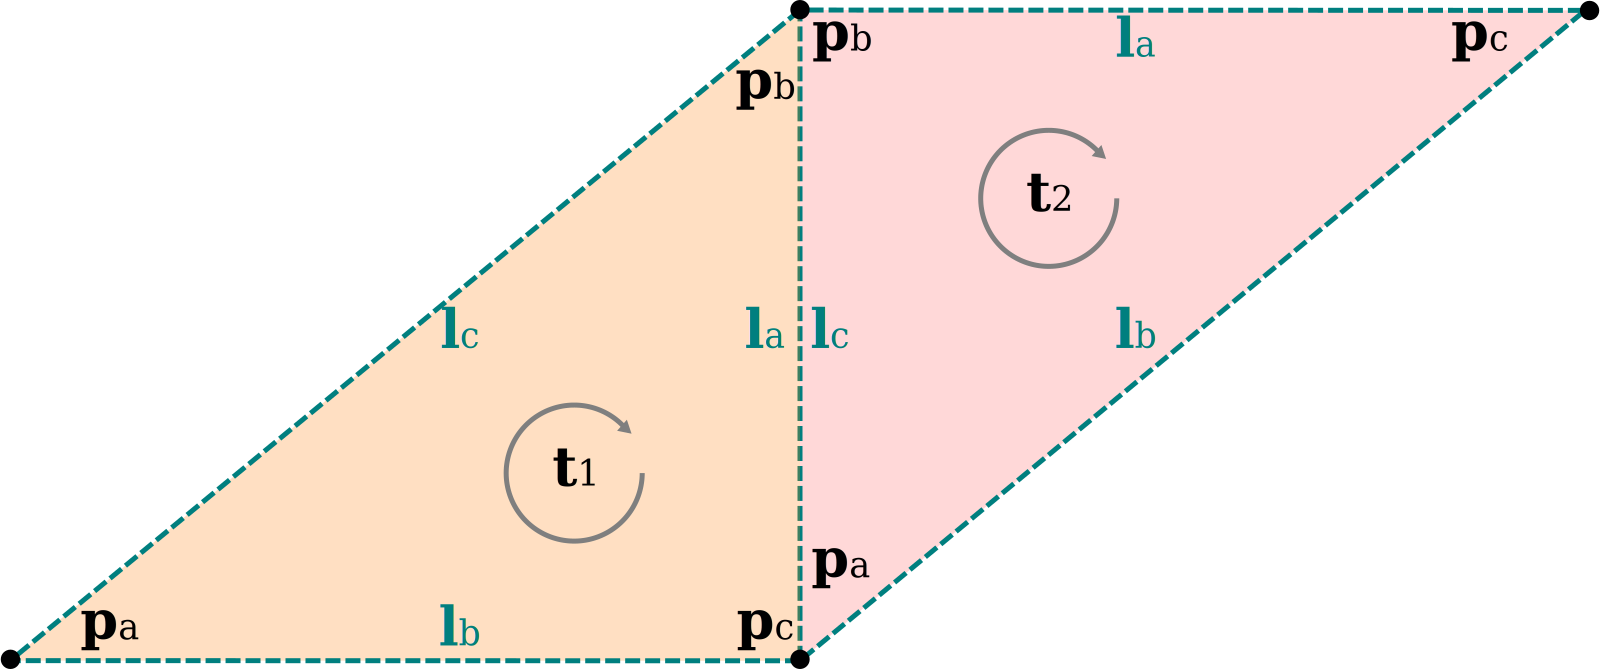
\includegraphics[width=1.0\linewidth]{figures/triangularFaces.png}}
	{\caption[Two Adjacent Triangular Faces]{Two adjacent triangular faces, $\bt_1$ and $\bt_2$, showing the relationship between their points, $\bp_a$, $\bp_b$, and $\bp_c$; their edge lengths, $\ell_a$, $\ell_b$, and $\ell_c$; and their clockwise orientation.}\label{fig:triangularFaces}}
\end{figure}

Each distinct triangular face is addressed using the global index $k$, and when taken together, comprise the set

\begin{equation}
	\bT := \left \{\:\bt_k \mid k \in \mathbb{N}, \;\text{and}\; 1\leq k \leq k_{max}\:\right \}
	\label{eq:defineSetOfFaces}
\end{equation}

where $k_{max}$ is the maximum index of faces in the data, and is equivalent to the cardinality of the set of faces $|\bT|$.%
\nomenclature[fa]{$\bT$}{the set of faces $\bt_k$ in $\bM$}%
\nomenclature[fb]{$\bt_k$}{a specific face in $\bT$}%

%
%
%
%
\subsection{Edge Lengths}
\label{ch2sTDDssEL}
As illustrated in Figure~\ref{fig:triangularFaces}, each triangular face is implicitly composed of three edges. Despite the fact that an edge is not typically\footnote{Other data structures, such as the Winged-Edge~\cite[p.~1]{Baumgart75}, may use edges as a primitive element} a primitive element of \tdd{}, we will endeavor to define the length of an edge $\ell$, because edge lengths are of particular significance for both the design and implementation of \fors{t}.

What is also particularly interesting about Figure~\ref{fig:triangularFaces}, is that when edge lengths are defined by the points of specific faces, each non-border edge length, illustrated in the figure as $\ell_a$ in $\bt_1$, and $\ell_c$ in $\bt_2$, will be labeled twice, despite representing the same distance.

When in the context of a particular face $\bt_k$, we will use a single index to define the length

\begin{equation}
	\ell_a := |\bp_b - \bp_c| \enspace:\enspace \left \{\,\bp_a,\,\bp_b,\,\bp_c\right \} = \bt_k
	\label{eq:defineEdgeLengthFace}
\end{equation}%
\nomenclature[ga]{$\ell_i$}{the length of the edge opposite the point $\bp_i$ of a specific face}%

and double indices when an edge length is referenced in relation to a specific point $\bp_v$ and its neighbor $\bp_i$

\begin{equation}
	\ell_{\sv{i}} := |\bp_i - \bp_v|
	\label{eq:defineEdgeLengthPoint}
\end{equation}%
\nomenclature[gb]{$\ell_{\sv{i}}$}{the length of the edge between points $\bp_v$ and $\bp_i$}%

Please be aware of the similar notation for the cardinality of a set $|\bP|$, to that for the calculation of the length of the edge $|\bp_i - \bp_v|$, as defined in Equation~\ref{eq:defineEdgeLengthPoint}. While cardinality is simply the count of elements in the set, the length is calculated as the L2-norm of the referenced vector~\cite[p.~26]{Mara12}.

\begin{equation}
\begin{aligned}
	|\bp_i - \bp_v| & = \lVert\bp_i - \bp_v\rVert_2 \\
					& = \sqrt{(x_i-x_v)^2 + (y_i-y_v)^2 + (y_i-y_v)^2}
	\label{eq:defineEdgeLengthCalc}
\end{aligned}
\end{equation}
\todoResearch{can I avoid sqrt altogether by performing entire algorithm squared?}

%
%
%
%
\subsection{Discrete Meshes}
\label{ch2sTDDssDM}
In \tdd{}, a mesh $\bM$ is the digital representation of a discrete manifold embedded in $\bR{3}$, and is typically\footnote{except in the case of specifically designed synthetic data, such as those presented in Section~\ref{ch6sSTDD}.} two-dimensional, non-planar and comprised of non-regular, triangular faces composed of connected points.~\cite[p.~25]{Mara12} A mesh is the set defined as

\begin{equation}
	\bM := \left \{\bP,\:\bT\right \}
	\label{eq:defineMesh}
\end{equation}%
\nomenclature[da]{$\bM$}{a mesh; the set including the sets of all points $\bp$ and faces $\bt$}%

with the set $\bP$ consisting of points, and the set $\bT$ consisting of triangular faces.

Many 3D-scanners produce point clouds\todoCitation{3D-scanners produce point clouds}, which as the name suggests, are comprised solely of a set of points $\bP$, and do not provide the set $\bT$. However, it is possible, and necessary for the production of a mesh, to perform a point set triangulation\todoCitation{perform a point set triangulation} in order to connect $\bP$ into a set of triangle faces, enabling one to combine the two sets into a mesh~\cite[p.~26]{Mara12}. For example, a portion of our experiments use a random triangulation disc generator, as presented in Section~\ref{ch6sSTDDssRTD}, which performs the well-known Delaunay triangulation\todoCitation{Delaunay triangulation} in order to produce a mesh from a randomly generated point cloud.
%\todoResearch{add figure of point cloud to triangulation}

%
%
%
%
\subsection{One-Ring Neighborhoods}
\label{ch2sTDDssORN}
It was mentioned in Section~\ref{ch2sETBssTsssN}, that it is a non-trivial task to determine the neighborhood of a point $\bp_v$, which exists in an irregular triangle mesh embedded in three dimensions. Having now examined the definitions of points, faces, and meshes, we can now formalize the one-ring neighborhood in \tdd{} as

\begin{equation}
	\bN_v := \left \{\;\bp_i\;:\;\left \{\,\bp_i,\,\bp_v\right \} \subseteq \bt \quad \forall \bt \in \bT\;\right \}
	\label{eq:defineNeighborhood}
\end{equation}%
\nomenclature[hb]{$\bN_v$}{the set of points comprising the one-ring neighborhood about $\bP_v$}%
\nomenclature[hc]{$\bp_i$}{a one-ring neighbor of $\bp_v$}%

In plain English, this means that the neighborhood $\bN_v$ is defined as the set of points $\bp_i$ such that both $\bp_i$ and $\bp_v$ are two points of a triangular face $\bt$, for all faces in the mesh. Therefore, the adjacency of points is defined by the co-membership within a face $\bt$, from the set of faces $\bT$.

When taken together, all the neighborhoods $\bN_v$ comprise a set of sets of neighbors; the family of sets

\begin{equation}
	\bN := \left \{\bN_v,\,\bN_{v+1},\ldots,\,\bN_{v_max}\right \}
	\label{eq:defineNeighborhood}
\end{equation}%
\nomenclature[ha]{$\bN$}{a family of sets of neighbors, the set of neighborhoods}%

This definition shares the indices $v$ and $v_{max}$ with the definition for a set of points, Equation~\ref{eq:defineSetOfPoints}, to highlight the fact that neighborhoods are defined per point. Therefore, there must be a correlation in the cardinality between the two sets.

Conversely, the cardinality of each individual neighborhood $|\bN_v|$ will likely vary among other neighborhoods in $\bN$. However, the value must always be $\geq 2$, and though there is no upper limit, $|\bN_v|$ is typically $\leq 12$. Furthermore, the neighboring points are always indexed in a clockwise direction for the same reasons as discussed in Section~\ref{ch2sTDDssF}.
%\todoResearch{get real upper limit for n}

As illustrated in Figure~\ref{fig:neighborhoods}, the set of black points are the neighbors $\bp_i$ which belong to the one-ring neighborhood\footnotemark $\bN_v$ centered on point $\bp_v$, which is drawn in coral color. The moniker originates from graph theory where each adjacent point is said to have a relative distance of one within the graph of the mesh. \footnotetext{A one-ring neighborhood can be extended to become a two-ring neighborhood by taking the union of the neighborhood $\bN_v$ with the neighborhood of each one-ring neighbor $\bp_i$, which adds to the neighborhood points with the relative distance of two within the graph. This iterative concept can be repeated k times and the neighborhood is then referred to as k-ring. Unfortunately, regardless of the fact that the relative distance within the graph can not be assumed equal to the geometric distance nor geodesic distance, it is still used throughout the literature, especially in the field of Computer Graphics~\cite[p.~29]{Mara12}.}
%\todoBackground{add a subsection on graph theory in basic theory section}

Our solution for maintaining a constant filter window size while convolving \fors{t} over neighborhoods of varying shapes and sizes is to determine the global minimum edge length, then use that as the radius of the geodesic disc centered at the central point of each neighborhood. Then when calculating the \wmfv{s} of each circle sector, using the interpolated function value from the neighboring points at the center of gravity. This process is explained in greater detail later in this thesis, and is the topic of Chapter~\ref{ch4}.

%
%
%
%
\subsection{Acquired versus Synthetic \tdd{}}
\label{ch2sTDDssAVS3}
The corpus of all \tdd{} exists in two flavors, acquired and synthetic data, with each being handily classifiable by the fashion in which it was generated, and the characteristics innate to those techniques.\todoReword{consider adding a figure here showing difference, or referencing a figure or pair of figures that does}

Acquired \tdd{} is typically captured as a point cloud utilizing various methods, such as: LiDAR (Light Detection and Ranging), Structured Light, or Structure from Motion~\cite[p.~19]{Mara12}. Then the data is exported from software packages accompanying the 3D-scanners as either just a point cloud comprised of a simple set of points $\bP$, or optionally as a triangle mesh $\bM$, described by one or more scalar-fields. Acquired \tdd{} also often consists upwards of a million points and as many as twice that number of faces\footnote{Appendix~\ref{apdx1} presents an interesting trend concerning how the ratio of face counts to point counts approaches to two for increasing mesh sizes, which is somehow related to Euler's polyhedron formula.}. These exported meshes~\cite[p.~25]{Mara12} uniformly contain noise and may exhibit other complexities for analysis, such as: non-manifold points, multiple borders and holes in the surface, inverted face orientation, non-manifold edges, and agglutination or degenerate faces~\cite[p.~28-32]{Mara12}.

Conversely, synthetic \tdd{} is artfully-crafted to avoid the complexities exhibited by acquired data. When modeling 3-dimensional objects, synthetic \tdd{} can require significantly less memory for storage, as simplifications can be made for large regular surfaces. For example, even the largest flat, rectangular surface can be modeled with only four points and two faces, whereas the acquired data methods require that the Nyquist–Shannon sampling theorem\todoCitation{Nyquist Shannon Theorem} be obeyed for the smallest detectable feature throughout the entire surface~\cite[p.~19]{Mara12}~\cite[p.~3]{Mara17}.

As presented in Section~\ref{ch6sSTDD}, for a portion of our experiments, we created another kind of synthetic \tdd{} which does not model a 3D-object. Instead, these synthetic-mesh generators produce different types of tessellations on arbitrarily large, planar surfaces, accompanied by a configurable scalar-field of function values.

%
%
%
\subsection{Function Values}
\label{ch2sTDDssFV}
In addition to the three Cartesian coordinates, points which comprise a mesh may also contain other relevant data in the form of scalar fields, or vector fields, when combined together into multi-dimensional data. This information, which is stored at each point $\bp$, often includes data regarding RGB color, material type, reflectivity, transparency, quality, confidence, or the resulting function values from an analytical filter such as \gls{tMSIIf}~\cite[p.~21]{Mara12}. A scalar field  can also be extended to include data important to other fields of study, such as infrared or ultraviolet light, temperature, rainfall, population, crime-rates, etc; essentially, any kind of data that may be measured at a point. As \fors{t} will currently\todoReference{future work/applications} only process a single field at a time, we can define a scalar field simply as the set of function values

\begin{equation}
	\bF := \left \{\: f_v \mid v \in \mathbb{N}, \;\text{and}\; 1\leq v \leq v_{max} \:\right \}
	\label{eq:defineSetOfFunctionValues}
\end{equation}%
\nomenclature[ia]{$\bF$}{the set of function values $f_v$; a scalar field}%
\nomenclature[ib]{$f_v$}{a specific function value in $\bF$, corresponding to $\bp_v$}%

This definition shares the indices $v$ and $v_{max}$ with Equation~\ref{eq:defineSetOfPoints}, the definition for a set of points, because it is indeed a fact that the cardinality of $|\bF|$ must be equal to $|\bP|$

\begin{equation}
	|\bF| \mbeq |\bP|
\end{equation}
g
because function values are only stored alongside the Cartesian coordinates, one-to-one with points, due to \tdd{} existing as a discrete manifold. The significance of which is another motivating factor behind the research conducted in this thesis.

%
%
%
%
%
%
\section{Parallel Processing}
\label{ch2sPP}
In this section, limited topics regarding the design and analysis of algorithms for parallel processing are briefly discussed, including: the nature of serial computation and threads; \gls{SIMD} as an architecture of concurrency; \glspl{GPGPU} as a tool for parallel processing; the identification of control and data dependencies in an algorithm; various topics regarding program correctness, including: the identification of critical sections, the utilization of mutexes as a locking mechanism, and the costliness of explicit thread synchronization; and finally the metrics available for evaluating a parallel algorithm.

%
%
%
%
\subsection{Serial Computation \& Threads}
\label{ch2sPPssSCT}
In a very general sense, when a computer executes a serial program, it proceeds one instruction at a time, sequentially in the order that it is written in the source code, and as required, reads from and writes to memory, which must then be reserved for it. Individually, these processes are called ``threads of execution'', or just ``\glspl{thread}'', and a single processing core can only process a single such thread at a time\footnote{This is not counting the limited application of parallel processing by exploiting the width of modern register arrays, in order to concurrently compute instructions at half or less precision.}.

Modern processors, however, can perform fast context switching\todoCitation{context switching}, which means loading the memory and state of a new thread, among a multitude of self-contained threads, and executing it so rapidly, as to give the illusion of parallel processing; similar to the commonly-known phenomenon where individual frames of film, when viewed at a high enough frequency, create the illusion of moving pictures\todoCitation{frame rates of movies}.

Fast context switching has its limitations, as even at the modern frequency of 4GHz\todoCitation{cpu benchmarks} per core, a serial algorithm can take dozens of hours, or even days, to finish computing, when iterating many times over a large collections of data, as seen in Section~\ref{ch6sCWGsCT}, the portion of our experiments comparing the timing of the serial version and the parallel variant of \fors{t} algorithm.

Alternatively, a system which exhibits some kind of architecture for real concurrency may execute programs which can then ``spawn'' new threads, which are given their own unique context, and thus may be run simultaneously on individual processing cores; enabling real parallel processing. One such architecture is discussed in the next section.

%
%
%
%
\subsection{SIMD - A Concurrency Architecture}
\label{ch2sPPssSACA}
All modern computers implement some form of parallelism, be it multi-core or multi-threaded processors, arrays of stream processors as found in GPUs, or the networks comprising supercomputers and data centers, and can therefore be classified by Flynn's Taxonomy of the different architectures of concurrency.\todoCitation{Flynn, 1966 doi:10.1109/TC.1972.5009071.}

Of the four classifications\footnote{\{SISD, SIMD, MISD, and MIMD\}} originally defined by Flynn, this thesis is primarily concerned with \glsreset{SIMD}\gls{SIMD}\footnote{or SIMT as is branded by NVIDIA.}\todoCitation{NVIDIA SIMT 4.1. SIMT Architecture} systems. As the name implies, the \gls{SIMD} classification is characterized by systems which are able to take a single instruction, otherwise known as a kernel\todoCitation{CUDA, kernels}, and execute it simultaneously on multiple elements from a pool of data. In general, this is described as ``processing in parallel''.

Figure~\ref{fig:simdArchitecture} illustrates a simplified impression of a system which employs SIMD architecture. The array of processors each receive the same kernel from a pool of instructions, then load a different portion of the data pool in order to process to combination in parallel.

\begin{figure}[ht]
\ffigbox
	{\includegraphics[width=1.0\linewidth]{figures/tikz/simdArchitecture.pdf}}
	{\caption[SIMD Architecture]{A simplified impression of a system characterized as SIMD by Flynn's Taxonomy of concurrent architecture. The array of processors each receive the same kernel from a pool of instructions, then load a different portion of the data pool in order to process the combination in parallel.}\label{fig:simdArchitecture}}
\end{figure}\todoCitation{Flynn, 1966 doi:10.1109/TC.1972.5009071.}

The motivation to implement software which utilizes the architecture of an \gls{SIMD} system is the speedup to be gained, which may be quantified as discussed in Section~\ref{ch2sPPssEAPA}, and stems from what is known as loop-level parallelism\todoCitation{loop level parallelism}, which is the modification of instructions which would otherwise be executed serially in a loop, to instead be computed simultaneously, in parallel, incurring only minor synchronization overhead. For example: any operation performed in linear algebra, such as the subtraction of two high-dimensional arrays, is thus made much more scalable in regards to the time required for the computation to complete, as vectors of larger and larger sizes are considered.

With the proper programming strategy, using the proper frameworks, the model for parallel processing on \gls{SIMD} architecture can be extended to far more complex instructions, and indeed, a major portion of the research presented in this thesis is focused on implementing the software to convolve the complex algorithm for \Fors{t}, by simultaneously executing its various kernels of instructions on every point and one-ring neighborhood in a mesh, in order to fully utilize the parallel architecture of an SIMD system; specifically, commercially-available \glspl{GPGPU}, which are described in the next section.

%
%
%
%
\subsection{GPGPU - General Use, Graphics Processing Unit}
\label{ch2sPPssGPGPU}
\glsreset{GPGPU}\gls{GPGPU} was coined by Mark Harris, the founder of GPGPU.org\todoCitation{Mark Harris, coined the term GPGPU}, and as the name implies, describes \glspl{GPU}, which was originally developed to exclusively perform graphics processing, but can now be utilized for general purposes by using the frameworks which are publicly available, for example OpenCL\todoCitation{OpenCL} and CUDA\todoCitation{CUDA}.

Figure~\ref{fig:cpuvgpu} illustrates the principle difference between a \gls{CPU}, and a GPU. Because graphics rendering is mostly comprised of compute-intensive, but highly-parallel procedures, \glspl{GPU} have been designed with less focus on data flow control and more transistors devoted to data processing\footnote{mimicking the design of early supercomputers}\todoCitation{LANG, footnote cray was a big GPU}. This diverges from the design of modern CPUs, which has devoted more chip space to processing at higher frequencies, while using large, multi-leveled caches of memory for the optimization of context switching\todoCitation{context switching}.

\begin{figure}[ht]
\ffigbox
	{\includegraphics[width=1.0\linewidth]{figures/cpuvgpu.png}}%{figures/tikz/cpuvgpu.pdf}}
	{\caption[CPU vs GPU Construction]{An illustration of the principle differences between a CPU and a GPU. CPUs have devoted more chip space to processing at higher frequencies, with more flow control and memory caching, while GPUs have been designed with more transistors devoted to data processing.}\label{fig:cpuvgpu}}
\end{figure}

%
%
%
%
\subsection{Control \& Data Dependencies}
\label{ch2sPPssCDD}
%Data Dependencies: ~\cite[p.~358]{Lang17}
%Data Partitioning:
%Calculations depend on specific data structures.~\cite[p.~357]{Lang17}
%As in edge lengths depend on the neighborhoods.

\todoResearch{https://en.wikipedia.org/wiki/Loop-level\_parallelism}
The concepts of control and data dependencies are not new ones, and can be dated back to the invention of multi-pass compilers\todoCitation{Data Dependencies and multi-pass compilers}. The field of study regarding the details is called dependence analysis and has far-reaching consequences from business management, to economics, as well as software optimization\todoCitation{dependence analysis}. In general, the basic concept behind both control and data dependencies is that some procedure A is said to be dependent on another procedure B, if A requires B to be executed first.

Figure~\ref{fig:simpleControlDependency} shows the ubiquitous if-then control structure as a simple example of a control dependency. It reads, ``if B is true, then do A''. In this case A is control dependent on B, because B must execute before it can be determined whether or not to execute A.

\begin{figure}[ht]
	\includestandalone[width=0.35\textwidth]{figures/tikz/simpleControlDependency}
	{\caption[If-Then Control Dependency]{A simple example of control dependency using the if-then control structure, with each distinct operation colored in teal, and control dependency marked with an arrow.}\label{fig:simpleControlDependency}}
\end{figure}

In the literature\todoCitation{4 kinds of data dependence}, there exist four distinct kinds of data dependence. Given that a certain value of data is stored in memory at a definite location and requires a finite amount of time to be read into context in order to be utilized by an operation, the four distinctions of data dependence are:
%
\begin{itemize}
	\item ``true dependence'', which is exhibited when one operation writes to a location in memory which is then later read from by another operation;
	\item ``anti dependence'', when one operation reads from a memory location later written to by a second operation;
	\item ``output dependence'', meaning that two operations are to write a data value to the same location in memory;
	\item and ``input dependence'', when two operations must read a value of data from the same location in memory.
\end{itemize}

In this thesis, we will generally not make distinctions between the various types, and will simply refer to any instance thereof as just ``data dependence''.

Figure~\ref{fig:dataDependencyOfL2Norm} illustrates the less-than-simple example of data dependencies inherent to calculating the L2-norm of a position vector in $\mathbb{R}^{3}$; an operation which will be revisited often in this thesis, and whose definition was already presented in Equation~\ref{eq:l2norm}. There are six individual procedures involved with calculating the L2-norm: three squarings, two additions, and one square root.

\begin{figure}[ht]
	\includestandalone[width=1.0\textwidth]{figures/tikz/dataDependencyOfL2Norm}
	{\caption[Data Dependencies in the L2-norm Calculation]{The data dependencies inherent to the calculation of the L2-norm of a position vector in $\bR{3}$, with each distinct operation colored in teal, and data dependencies marked with arrows. The centered block in sand color represents an exclusive-or situation, abbreviated as xor, where one, and only one pair of operations shall execute.}\label{fig:dataDependencyOfL2Norm}}
\end{figure}

The three squaring procedures are totally independent of each other and can be performed in any order, indeed even concurrently, in relation to one another. In contrast, the two additions are totally dependent on their addends, because while the order in which the first two of the three addends are used is inconsequential due to the commutative property of addition, the first addition is always dependent on the completion of two squarings, and the second addition is dependent on not only the sum from the first addition, but also the product of the third squaring. Finally, because the square root procedure is dependent on the execution of both additions, it inherits their dependencies on the squaring procedures, and therefore must wait until the very end before executing last.

A proper understanding of all dependencies becomes even more crucial when designing software which processes data in parallel, because it is no longer implicitly-known when a particular operation has completed, so that the dependent operation may begin. Managing those complications is the topic of the next section.

%
%
%
%
\subsection{Program Correctness}
\label{ch2sPPssPC}
\Gls{programCorrectness}, which may otherwise be referred to as functional correctness, is defined by the field of theoretical computer science as existing only when, for each input given, a program produces the expected output\todoCitation{definition of program correctness}. In this section, we discuss the dangers inherent to asynchronous parallel processing, mentioning the concepts of critical sections, the mutex locking mechanism, and the explicit synchronization of threads.

%
%
\subsubsection{Critical Sections}
\label{ch2sPPssPCsssCS}
One major consequence of processing in parallel is that, due to the independence enjoyed by individual threads, the sequence in which operations are performed can no longer always be guaranteed. That is not intrinsically a problem, however, it becomes a critical issue with the introduction of data dependence, which requires that information be shared among threads by reading from and writing to \gls{volatileMemory}, which is memory that may be changed by any thread without warning.

Sections of code containing the instructions that utilize volatile memory are aptly named ``\gls{criticalSection}'', and special care must be taken in their regard, in order to ensure program correctness, despite not being able to determine in what order the operations may occur.

For an illustrative example, consider Algorithm~\ref{alg:critialSection}, the very simple parallel program to compute the sum of a set of integers. Given the set $\{1,\,2,\,3,\,4\}$, the function \textit{parallelSum} instantiates the value $s$ as zero, in order to later accumulate the sum calculated in each thread, then spawns two threads, which each execute the kernel \textit{accumulateSums} with a unique subset of the work to be done. Each kernel then simultaneously adds the two integers, naively reads the current value of $s$, adds the sum to that value, then stores the result back into $s$.

\begin{algorithm}[ht]
	\DontPrintSemicolon
	\SetCommentSty{small}
	\SetKwFor{For}{for}{:}{}
	\SetKwProg{Func}{Function}{}{}
	\SetKwProg{Kernel}{Kernel}{}{}
	\SetKwInOut{Input}{Input}\SetKwInOut{Output}{Output}

	\Input{the set of integers $\{1,\,2,\,3,\,4\}$}
	\Output{the sum $s$}

	\bigskip
\nl	\Func{parallelSum($\{1,\,2,\,3,\,4\}$)}{
\nl		$s \leftarrow 0$\;
\nl		\ProgSty{$\sim$sum($s$, 1, 2)}\;
\nl		\ProgSty{$\sim$sum($s$, 3, 4)}\;
	}

	\bigskip
\nl	\Kernel{accumulateSums($s$, $a$, $b$)}{
\nl		$s' \leftarrow a + b$\;
\nl		$s \leftarrow s + s'$\tcc*{Danger!}\label{algCritSec.danger}
	}
	\caption{Simple parallel algorithm, exhibiting an unprotected critical section \label{alg:critialSection}}
\end{algorithm}%

Unfortunately, the final result of the execution of function \textit{parallelSum} can not be accurately predicted, because the order of operations between each thread are not guaranteed due to what is known as a ``\gls{raceCondition}'' in the algorithm. Closer evaluation of line~\ref{algCritSec.danger} reveals the danger of the \gls{raceCondition} inherent to this \gls{criticalSection}.

The high level code in line~\ref{algCritSec.danger} will be translated by a compiler into low level assembly instructions\todoCitation{LANG pg 25} written in Algorithm~\ref{alg:critialSectionLowLevel}, which are then executed in parallel by both threads.

\begin{algorithm}[ht]
	\DontPrintSemicolon
	\SetCommentSty{small}
\nl	R1 $\leftarrow s$\;
\nl	R2 $\leftarrow s'$\;
\nl R3 $\leftarrow$ ADD R1 R2\;
\nl	$s \leftarrow$ R3\;
	\caption{A low level translation of the critical section in Algorithm~\ref{alg:critialSection} \label{alg:critialSectionLowLevel}}
\end{algorithm}%
\todoStyle{make this alg block less formal}

Figure~\ref{fig:raceCondition} illustrates how, because the value $s$ is in volatile memory which is shared by both threads, and because each thread remains independent, performing their instructions sequentially at their own speeds, the total order of operations can not be guaranteed and will fall within a range of limited permutations. The consequence being, that only one third of the possible outcomes are actually correct, producing the sum of the four integers as would be expected.

\begin{figure}[ht]
\ffigbox
	{\includegraphics[width=0.8\linewidth]{figures/tikz/raceCondition.pdf}}
	{\caption[A Simple Race Condition]{the possible permutations of operations as outcome of accumulating a sum with parallel threads without mutual exclusion. The two teal color paths are the only produce correct results, while the four coral colored paths produce only a partial sum.}\label{fig:raceCondition}}
\end{figure}

In order to manage the complications inherent to the \glspl{raceCondition} engendered by the presence of \glspl{criticalSection} in code processed in parallel, it becomes necessary to introduce some type of locking mechanism with which one can control the flow of execution with regards to data dependence. The one and only type of locking mechanism used in this thesis, the mutex, is discussed in the next section.

%
%
\subsubsection{Mutexes}
\label{ch2sPPssPCsssM}
The term ``\gls{mutex}'' is an abbreviation for ``mutual exclusion'', which is used to describe the situation where the presence of a single entity may exclude the presence of all others. For parallel processing, that translates to allowing only one single thread to enter a critical section of code at a time. A mutex is typically implemented as a shared value which any thread wanting to enter a critical section in code must first find unlocked, before locking the mutex itself and performing the operations therein. All other threads wanting to also enter the critical section will find the mutex locked, and therefore must ``block'', waiting until the mutex is again unlocked, before being able to proceed.

While it is true that employing a mutex can be expensive to both compute time and memory\todoResearch{how expensive are locking mechanisms} because blocking intrinsically means the cessation of computation, however, when used efficiently, the speedup gained by exploiting the parallelism of an algorithm becomes worth the cost\todoResearch{quantify the cost} of the added synchronization overhead.~\cite[~p.20]{Lang17} An example of this is thoroughly explored in the description of Algorithm~\ref{alg:parallelConvolveFilter}, and the effects of this overhead can be seen in the results of the timing experiments presented in Sections~\ref{ch6sCWGssS}~and~~\ref{ch6sCWGssE}, later in this thesis.

%
%
\subsubsection{Explicit Thread Synchronization}
\label{ch2sPPssPCsssETS}
Occasionally, in order to maintain the correctness of the overall program due to some dependence within the code, an algorithm is forced to block, waiting for all threads to complete their calculations, before finally continuing with its computations. This procedure is called, ``\gls{explicitSynchronization}'',\todoCitation{CUDA 3.2.5.5.3. Explicit Synchronization} and is expressed in the parallel algorithms presented in this thesis by a call to the subroutine \textit{synchronizeThreads}.

Explicitly synchronizing threads can be very expensive, costing the overall efficiency of an algorithm greatly; easily reaching the level of billions of compute cycles.\todoResearch{get stats on thread synch}\todoReference{experiments about thread synch time costs}. Therefore, it is absolutely imperative that one minimizes its inclusion in the design of any parallel algorithm, especially within loops, avoiding it altogether whenever possible\todoResearch{avoiding thread synch}, and limiting its use to only the sections of an algorithm which signify the culmination of a large volume of parallel work.

In this section, we discussed the dangers to program correctness that are inherent to parallel processing, including the concepts of \glspl{criticalSection} which arise when individual threads must share information via volatile memory, the mutex locking mechanism which can be used to protect critical sections in order to preserve program correctness, and the explicit synchronization of threads which can be very expensive to the overall efficiency of an algorithm. In the next section, we will explore a few of the metrics that can be used to evaluate and analyze parallel algorithms, for use in comparison and possible further optimization. \todoReword{maybe dot suggest how to use it, also 'ways' instead of metrics.}

%
%
%
%
\subsection{Evaluation and Analysis of Parallel Algorithms}
\label{ch2sPPssEAPA}
When engaging in the design of parallel algorithms, it is useful to define metrics which can be used to quantitatively describe the differences engendered by the modifications made to the basic serial algorithm. Such metrics could then influence not only choices in the design, but also environments under which the algorithm should be run. For example, in answering the question regarding the scalability of the algorithm and the worthiness of incurring the costs of increasing the count of processors in the pursuit of faster computation times~\cite[p.~330]{Lang17}.
\todoReword{recap each paragraph}

Timing is essential to every metric used in the evaluation of parallel algorithms. Given the inputs, $\hat{n}$ as the number of operations to be performed by the algorithm, and $\rho$ as the count of processors available in the system, one can define the two essential timings as:

\begin{align}
	\mathit{T_s}(\hat{n}) &= \text{The optimal sequential execution time} \\
	\mathit{T_{\rho}}(\hat{n},\,\rho) &= \text{Parallel runtime}
	\label{eq:timings}
\end{align}

which can then be used to define the three essential metrics:

\begin{align}
	\text{\Gls{speedup}:}\quad&\mathit{S}(\hat{n},\,\rho) = \frac{\mathit{T_s}(\hat{n})}{\mathit{T_{\rho}}(\hat{n},\,\rho)} \\
	\text{Costs}:\quad&\mathit{C}(\hat{n},\,\rho) =\rho\cdot\mathit{T_{\rho}}(\hat{n},\,\rho) \\
	\text{\Gls{efficiency}}:\quad&\mathit{E}(\hat{n},\,\rho) = \frac{\mathit{T_s}(\hat{n})}{\mathit{C}(\hat{n},\,\rho)} = \frac{\mathit{S}(\hat{n},\,\rho)}{\rho}
	\label{eq:essentialMetrics}
\end{align}
\todoReword{write significance, in regards to experiments and evaluation}

By applying these identities, we can determine that for all problem sizes, the \gls{speedup} obtained is always less than the number of processors used, because otherwise, $\mathit{T_s}(\hat{n})$ could not be the optimal sequential execution time. Also, \gls{efficiency} will always be less than one thus we can say that $\mathit{E}\cdot\rho$ processors contribute to the solution of the total procedure, while $(1-\mathit{E})\cdot\rho$ do not~\cite[p.~335]{Lang17}.

Also important is the notion of an algorithm's ``\gls{degreeOfPar}'', which is the maximum number of operations that can be executed in parallel, a principle central to \gls{Amdahl}\todoCitation{Amdahl's Law}, which is defined as, when given a constant problem size $\hat{n}_{fixed}$, and an algorithm's \gls{degreeOfPar} $q$,

\begin{equation}
	\lim_{\rho \to \infty} \mathit{S}(\hat{n}_{fixed},\,\rho) = 1 / q
\end{equation}

This leads to the conclusion that one can not simply add more processors in order to gain appreciable speedup, but instead that relies heavily on processor counts which grow in relation to problem sizes, and the degree of parallelism, which itself relies on the underlying nature of the serial algorithm and the artful design of the parallel algorithm.

%, each with their own unique ids and memory addresses,

%As memory to be processed by a thread is stored somewhere in a hierarchy which increases in size, but decreases in speed as one moves from the processor's registers, it is likely that a context switch will cause what is known as a cache miss\todoCitation{cache hit or miss, check Lang}, which incurs a time penalty while the processing stalls and the required memory is read from slower hardware sources.

%\subsection{Host Memory and Device Memory}
%\todoBackground{memory vs speed}
%Hardware consists of memory and processors. Memory is divided into a hierarchy which starting at the registers on the processors themselves, increases in capacity, but decreases in speed.\todoReword{moves away from} Of particular interest to this thesis...\todoReword{continue}


%\subsection{Hardware Implementation}%4. Hardware Implementation}
%\section{CUDA extended C++: An interface for GPGPU implementation}
%\subsection{CUDA C Runtime}%3.2. CUDA C Runtime}
%\subsection{Versioning and Compatibility}%3.3. Versioning and Compatibility}
%\subsection{Versions <9, vs >= 9}
%
%\subsection{Iso-efficiency}
%	WK(P) = iso-efficient if it fulfills:
%	TO(WK(P), P) = KWK(P)~\cite[p.~350]{Lang17}
%
%\subsection{Scalability}
%	A parallel system is called scalable only if in has an iso-efficency function

%
%
%
%
%
%
\section{Summary}
This chapter briefly covered many topics across many fields of study, opting for breadth over depth in order to focus only on the specific topics which have a direct influence on research presented in the rest of this thesis.

Section~\ref{ch2sETB} covered the elementary, theoretical basis for the mathematics utilized in the design of \fors{t}, including various topics in set theory, linear algebra, geometry, and topology. We delved into: expressing definitions, special sets, cardinality, as well as selected membership, relational, and binary operators; position vectors, the subtraction of vectors, and computing the L2-norm; geodesic discs, circle sectors, centroids and the center of gravity, and interpolation and extrapolation; as well as manifolds and neighborhoods.

Next, Section~\ref{ch2sTDD} defined several symbols which will be used throughout the rest of this thesis. It discussed in relative detail, the primitives of \tdd{}: points, faces, and edge lengths, as well as the nature of discrete meshes, one-ring neighborhoods, the differences between acquired and synthetic \tdd{}, and the treatment of scalar fields as function values.

Then in Section~\ref{ch2sPP}, limited topics regarding the design and analysis of algorithms for parallel processing were briefly presented. These included: the nature of serial computation and threads; SIMD as an architecture of concurrency; GPGPUs as tools for parallel processing; the identification of control and data dependencies in an algorithm; various topics regarding program correctness, including: the identification of critical sections, the utilization of mutexes as a locking mechanism, and the costliness of explicit thread synchronization; and finally the metrics available for evaluating a parallel algorithm.

In the next three sections, we will present \Fors{t}. This begins with the mathematical foundations upon which the the filter was designed, then we present the three parts of the serial algorithm for convolving the filter over a discrete manifold, and we conclude with an analysis of the serial algorithm, and the presentation of a parallel variant of each of its parts.

